\documentclass[mathserif]{beamer}

%% Packages section
\usepackage[utf8]{inputenc}
\usepackage{graphicx}
\usepackage{tikz}
%% \usepackage{caption}
\newcommand{\myfig}[2] {
  \begin{figure}[!h]
    \centering
    \includegraphics[scale=#1]{#2}
  \end{figure}
}

%% Options section
\usetheme{Boadilla} 
\useinnertheme[shadow]{rounded}
\usecolortheme{dolphin}
\useoutertheme{infolines}

\title{Monitoring du noyau Linux}
\subtitle{sur une architecture NUMA}
%% \subtitle{Sous la direction de Gaël Thomas}
\author[Gallardo - Lombardet - Peneau]{Kevin Gallardo\\Eric Lombardet\\Pierre-Yves Péneau}

\newcommand{\bframe}{\begin{frame}{\secname}{\subsecname}}

\date{12 Mai 2014} \institute[UPMC]{Université Pierre et Marie
  Curie}

\begin{document}

  %% \captionsetup[figure]{labelformat=empty}

  \frame{\titlepage}

  \section{Introduction}
    \bframe
      \begin{itemize}
        \item problématique:\newline \vspace{0.2cm}\hspace{0.4cm} architectures
          NUMA, placement mémoire, performances\newline
        \item<2> objectif:\newline \vspace{0.2cm}\hspace{0.4cm} évaluation
          d'activité, mesures d'évènements, étude comportementale
        \end{itemize}
    \end{frame}

  \section{Architecture NUMA}
    \subsection{Présentation}

      \bframe
        \visible<1-> {
          \begin{block}{Objectifs}
            \begin{itemize}
              \item accélerer les temps de traitement
              \item répondre aux besoins d'applications spécifiques
            \end{itemize}
          \end{block}
        }
        \visible<2-> {
          \begin{block}{Moyens mis en \oe uvre}
            \begin{itemize}
              \item découpe en noeuds
              \item placement des contrôleurs d'E/S
              \item liens d'interconnexions
              \item mise en place d'une topologie
            \end{itemize}
          \end{block}
        }
      \end{frame}

    \subsection{Vue d'ensemble}
      \bframe
        \myfig{0.4}{img/numa_arch_details.png}
      \end{frame}

    \subsection{Enjeux}
      \bframe
        \begin{itemize}
          \item placement mémoire
          \item placement des threads
          \item activité d'entrées/sorties
        \end{itemize}
        \myfig{0.4}{img/topo.png}
      \end{frame}

  \section{Infrastructure de tests}
    \subsection{}
      \bframe
        \begin{itemize}
          \item utilisation mutualisée du Magny Cour $\rightarrow$ machines
            virtuelles
          \item problème: pas d'IBS avec qemu
        \end{itemize}
      
        \visible<2-> {
          \begin{alertblock}{Conséquence}
            Travail en réel sur le noyau pour 50\% du projet
          \end{alertblock}
        }
      \end{frame}

  \section{Monitoring}
    \subsection{Qu'est-ce que c'est ?}
      \bframe
        \begin{itemize}
          \item étude bas niveau du comportement matériel et système
          \item très utile pour le débugage ou l'optimisation poussée
          \item différentes solutions de monitoring existent
        \end{itemize}
      \end{frame}

    \subsection{Instruction Based Sampling - Présentation}
      \bframe
        \begin{itemize}
          \item technologie AMD
          \item informations plus précises car spécifique à une famille de
            processeur
          \item problème:w
            \begin{itemize}
              \item plus difficile à mettre en place
            \end{itemize} 
        \end{itemize}
      \end{frame}

    \subsection{Instruction Based Sampling - Fonctionnement}
      \bframe
        \begin{itemize}
          \item tag aléatoirement une instruction
          \item suivi de l'exécution
          \item deux types de mesures: fetch/execution sampling
        \end{itemize}
      \end{frame}

    \subsection{Instruction Based Sampling - Utilisation}
      \bframe
        \begin{itemize}
          \item<1-2> beaucoup d'informations remontées par IBS
          \item<1-2> sélection des plus utiles: cache hit/miss
        \end{itemize}

        \visible<2->{
          \begin{figure}[h]
            \centering
            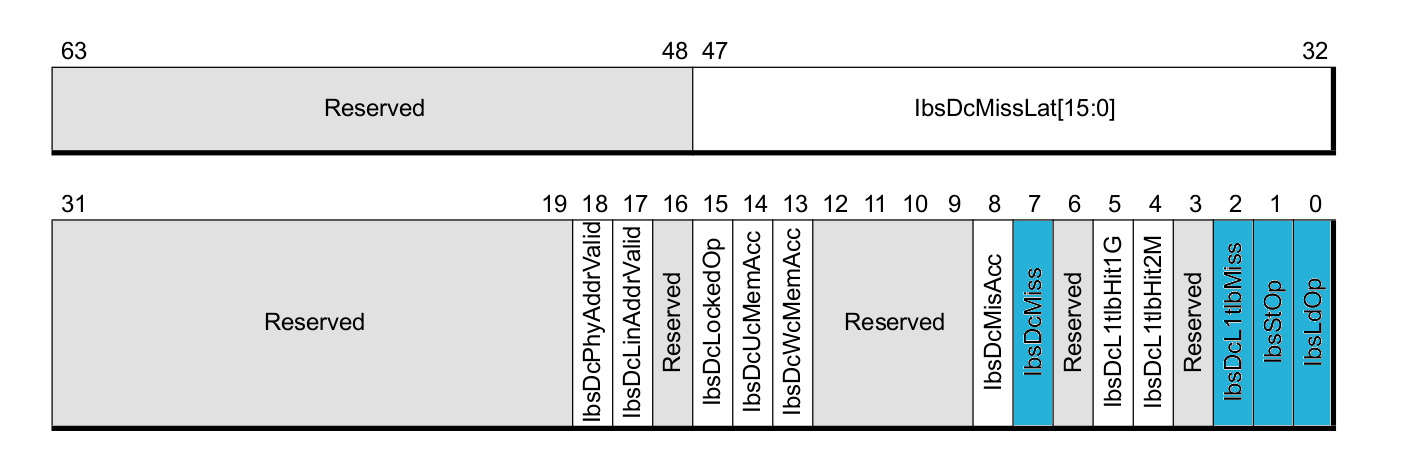
\includegraphics[scale=0.22]{img/data3_color.png}
            \caption{Schéma du registre MSR IbsOpData3}
          \end{figure}
        }
      \end{frame}

    \subsection{Instruction Based Sampling - Défauts}
     \bframe
       \begin{itemize}
         \item overhead: traitement coûteux des mesures
         \item pas de vision d'ensemble
       \end{itemize}
     \end{frame}

    \subsection{Mise en place}
      \bframe
        \begin{itemize}
          \item configuration de l'APIC
          \begin{itemize}
            \item informer l'APIC de la présence d'interruptions IBS
            \item à faire pour chaque coeur
          \end{itemize}
          \item enregistrement d'un handler NMI
          \begin{itemize}
            \item appelé à chaque interruption IBS
            \item récolte les informations dans les registres MSR
          \end{itemize}
        \end{itemize}
        \visible<2->{
          \begin{alertblock}{Attention}
            le handler doit être enregistré une et une seule fois au niveau du système
          \end{alertblock}
        }
      \end{frame}

  \section{Mesures sur le noyau Linux}
    \subsection{Chaleur d'un thread}
      \bframe
        \begin{itemize}
          \item un compteur représente l'activité d'un thread
          \item différents critères d'activité:
            \begin{itemize}
              \item état: (in)actif
              \item taux d'utilisation mémoire
              \item nombre d'entrées/sorties
              \item commnunications entre threads
              \item \ldots
            \end{itemize}
        \end{itemize}
      \end{frame}

    \subsection{Méthodes de tri envisagées}
      \bframe
        \begin{itemize}
          \item nécessité d'une structure dédiée
          \item utilisation d'un tableau ou d'une liste chainée
          \begin{itemize}
            \item insertion de nouveaux threads
            \item difficulté à trouver les threads morts
            \item tri peu performant
          \end{itemize}
        \end{itemize}
        \visible<2-> {
          \begin{alertblock}{Conclusion}
            Solution abandonnée
          \end{alertblock}
        }
      \end{frame}

      \bframe
          Utilisation d'un tableau de chaleur
          \myfig{0.9}{img/screen1.png}
      \end{frame}
      \bframe
          Utilisation d'un tableau de chaleur
          \myfig{0.9}{img/screen2.png}
      \end{frame}
      \bframe
          Utilisation d'un tableau de chaleur
          \myfig{0.9}{img/screen3.png}
      \end{frame}
      \bframe
          Utilisation d'un tableau de chaleur
          \myfig{0.9}{img/screen4.png}
      \end{frame}

    \subsection{Solution retenue}
      \bframe
        \begin{itemize}
          \item ajout du compteur dans la task\_struct
          \item on conserve le tableau de chaleur précédent
          \item structure Gestion pour les listes
        \end{itemize}
        \myfig{0.3}{img/screen5.png}
      \end{frame}

      \bframe
        \myfig{0.33}{img/screen6.png}
      \end{frame}

    \subsection{Réalisation}

      \bframe
        Algorithme:
        \begin{itemize}
          \item[1] stopper IBS
          \item[2] vider le tableau de chaleur
          \item[3] parcour la task\_struct
          \begin{itemize}
            \item[a] si RUNNING $\rightarrow$ incrémentation du compteur de chaleur
            \item[b] sinon décrémentation
          \end{itemize}
          \item[4] générer le tableau de chaleur
          \item[5] lancer les mesures sur ls threads chauds
        \end{itemize}
      \end{frame}

      \bframe
        \begin{block}{Optimisation}
          \begin{itemize}
            \item Utilisation d'un facteur d'incrémentation et de décrémentation
              dynamique
          \end{itemize}a
        \end{block}
        \visible<2-> {
          \begin{alertblock}{Problèmes}
            \begin{itemize}
            \item pas d'IBS avec qemu
            \end{itemize}
          \end{alertblock}
        }
      \end{frame}

  \section{Conclusion}
    \bframe
     20/20 ou chinois tuer et manger ta famille !
     \begin{figure}[h]
       \centering
       
\includegraphics[scale=0.4]{img/jackiechan.jpg}\newline
       \textit{``Tu veux un bol de riz ?''}
     \end{figure}

    \end{frame}

\end{document}
